\textbf{See the instruction for questions \inteval{\value{question}+1} to \inteval{\value{question}+2}.}

\begin{figure}[H]
    \centering
    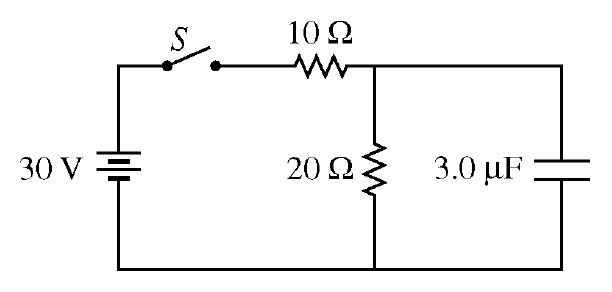
\includegraphics[scale=0.5]{images/24.25.png}
\end{figure}

An uncharged $3.0 \mu \mathrm{F}$ capacitor is placed in a circuit with an ideal battery, two resistors, and an open switch $S$, as shown in the figure above. The switch is then closed.

% Multiple Choice Question 24
\begin{questions}\setcounter{question}{23}\question
What is the current in the $10 \latinunit\Omega$ resistor immediately after the switch is closed?

\begin{oneparchoices}
\choice Zero
\choice $1.0 \unit{A}$
\choice $1.5 \unit{A}$
\choice $3.0 \unit{A}$
\choice $10 \unit{A}$
\end{oneparchoices}\end{questions}

% Multiple Choice Question 25
\begin{questions}\setcounter{question}{24}\question
What is the current in the $20 \latinunit\Omega$ resistor a long time after the switch is closed?

\begin{oneparchoices}
\choice Zero
\choice $1.0 \unit{A}$
\choice $1.5 \unit{A}$
\choice $3.0 \unit{A}$
\choice $10 \unit{A}$
\end{oneparchoices}\end{questions}
